\section{Задачи машинного обучения}
Supervised и unsupervised. Регрессия, классификация, кластеризация. Метрики качества.
Рассмотрим типы задач, которые встречаются в машинном обучении.

\subsection{Классификация}
Рассмотрим следующую задачу. Мы работаем в банке и нам необходимо, чтобы система определяла, сможет ли человек вовремя погасить кредит или нет. 

У нас есть различная информация о человеке, так называемые \textbf{признаки (features)}. Они бывают различных типов:
\begin{itemize}
    \item \textbf{Бинарные признаки}: наличие телефона.
    \item \textbf{Номинальные признаки}: профессия, адрес проживания.
    \item \textbf{Порядковые признаки}: образование, занимаемая должность. По сути, они похожи на номинальные признаки, только тут у значений признака имеется порядок (высшее образование ценится выше среднего и т.д.).
    \item \textbf{Количественные признаки}: зарплата, возраст, количество детей в семье и т.п.
\end{itemize}

Ответ же к данной задаче либо \textbf{0} (человек не выплатит кредит вовремя) и \textbf{1} (Человек выплатит кредит вовремя).

Т.е. в задаче классификации значение, которое мы хотим предсказать (далее целевая переменная ), принадлежит конечному множеству. В нашей задаче, например, это \textbf{\{0; 1\}}. 

Бывают множества не только из 2 классов. Например, задача диагностики болезни по симптомам. Тут классы — это список болезней.

Как решается данная задача? В таких задачах нам требуется \textbf{обучающая выборка}. Это история того, как в прошлом наши клиенты выплачивали кредиты.

Мы знаем о них все: где они работают, сколько получают и т.п. А также нам известно смогли они выплатить кредит или нет. 

Знание того, что мы предсказываем (целевой переменной) относит задачу к \textbf{обучению с учителем}.

Далее модель машинного обучения находит закономерности в этой выборке. Например, если человек безработный, то скорее всего, он не выплатит кредит вовремя и т.д. 

Она запоминает эти закономерности, и когда приходит черёд узнать, а сможет ли новый клиент заплатить кредит вовремя, модель смотрит на эти зависимости и выдаёт ответ. 

Список новых клиентов называется \textbf{тестовой выборкой}. Главное её отличие от обучающей выборки заключается в том, что для элементов из тестовой выборки неизвестна целевая переменная (в нашем случае — это выплатит клиент кредит или нет).

\subsection{Регрессия}
Еще одним типом является \textbf{регрессия}. 

Например, можно рассмотреть такую задачу: мы хотим по росту родителей определить насколько высоким может быть их ребёнок. Действительно, как правило, есть зависимость, что у высоких родителей дети тоже имеют высокий рост и наоборот. 

Т.е. от классификации задача регрессии отличается тем, что тут целевая переменная — вещественное число.

\textbf{Обучающей выборкой} в данной задаче будет набор троек: (рост родителя №1, рост родителя №2, рост ребёнка). 

\textbf{Тестовой выборкой} — набор двоек: рост родителя №1 и рост родителя №2.

\subsection{Кластеризация}
В обучающих выборках, рассмотренных выше задач, нам была известна целевая переменная:
\begin{itemize}
    \item Выплатит ли человек кредит вовремя — в задаче классификации
    \item Рост ребенка — в задаче регрессии.
\end{itemize}

\newpage{}

Однако, целевая переменная не всегда известна. Например, мы провели социологический опрос, у нас есть много ответов на вопросы и нам хотелось бы сгруппировать их по поведению. Мы заранее не знаем, сколько таких кластеров получится и что они из себя представляют. Это мы можем узнать только после того как появятся сами кластеры.

Еще простой и пробирочной задачей кластеризации является кластеризация точек на плоскости
\begin{center}
    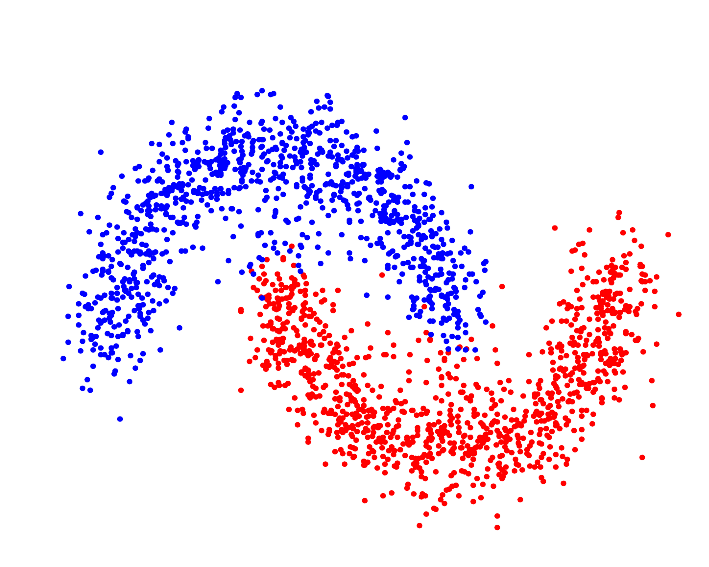
\includegraphics[scale=0.5]{tickets/pictures/make_moons.png}
\end{center}